\section {Étude analytique du projet}

Ce chapitre présentera les outils utilisés pour la réalisation de la conception de notre projet. Par ailleurs, il relate ses différentes étapes, ainsi que les diagrammes dégagés après chaque étape.

\subsection {Diagramme des packages}
\subsubsection{Définition}
Le diagramme des packages est un diagramme UML qui fournit une représentation graphique de haut niveau de l'organisation de l’application à réaliser.
\subsubsection{Diagramme des packages du projet}
De prime abord, il convient de distinguer les différents modules à développer dans le cadre du projet. Ainsi le diagramme de packages illustré dans la figure 5 ci-après montre clairement les trois modules à mettre en jeu.
\begin{figure}[!h]
	   \center
	   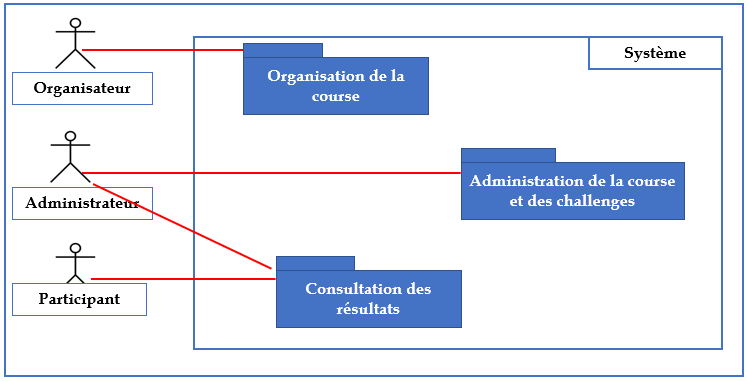
\includegraphics[scale=0.9]{img/Diagramme_de_packages.png}
	   \caption {Diagramme de packages du projet}
\end{figure}

Ce diagramme permet de dégager trois packages principaux qui seront détaillés dans le cadre des cas d’utilisation illustré dans l’axe suivant.

\subsection {Les cas d’utilisation}

\subsubsection{Définition}
Les cas d'utilisation sont définis par une description textuelle, décrivant les objectifs et interactions entre le système et ses acteurs. Le format de présentation textuelle des cas d'utilisation est libre.
\subsubsection{Diagramme de cas d’utilisation }
Comme illustré par le diagramme des packages, trois modules sont à développer. Ces modules nécessitent l’élaboration de trois cas d’utilisation. Le premier cas d’utilisation du projet traite de la phase de l’organisation d’une course (tel montré sur la figure ci-dessous). En effet le seul acteur qui interagit avec le système dans ce cas est l’organisateur de la course. Ainsi le système doit permettre de réaliser un certain nombre de fonctionnalités qui sont répertoriées comme suit :
\begin{itemize} 
\item La saisie des données des participants dans une course
\item  L’établissement du classement des participants dans la course
\item  L’envoi des résultats finaux à la ligue pour permettre à l’administrateur de mettre à jour le fichier des challenges.
\end{itemize} 

\begin{figure}[!h]
	   \center
	   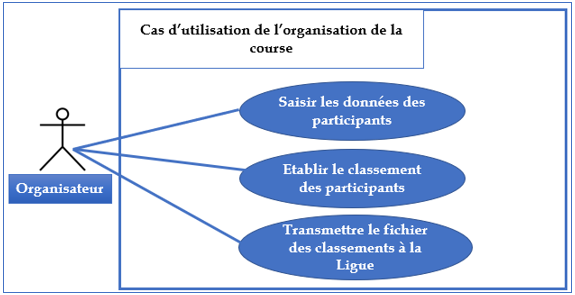
\includegraphics[scale=0.9]{img/Diagramme_cas_utilisation_organisation_course.png}
	   \caption {Diagramme de cas d’utilisation relatif à l’organisation d’une course}
\end{figure}


S’agissant de l’étape de l’administration, l’acteur qui utilise le système est l’administrateur de la ligue. Dans ce cas l’administrateur doit pouvoir effectuer les tâches suivantes :
\begin{itemize} 
\item Valider les fichiers des courses envoyés par les organisateurs des courses (Supprimer les participants qui ne sont pas inscrits dans la ligue, traiter les homonymes…) ;
\item Créer le fichier challenge, s’il n’existe pas et le mettre à jour ;
\item  Consulter les résultats et les statistiques inhérentes aux courses selon un certain nombre de critères de choix (comme les clubs, les catégories…).
\end{itemize} 

\newpage
Ainsi la figure ci-dessous illustre clairement le cas d’utilisation de cette étape.

\begin{figure}[!h]
	   \center
	   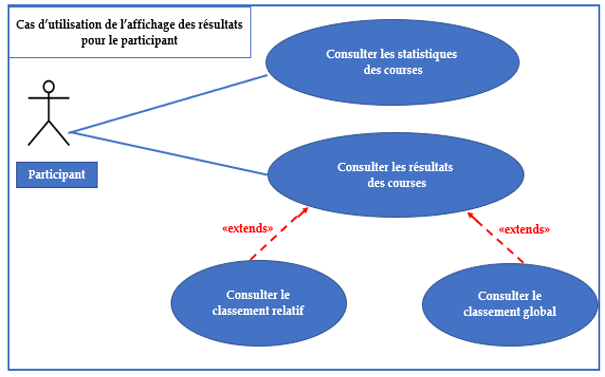
\includegraphics[scale=0.9]{img/Diagramme_cas_utilisation_administration_challenge.png}
	   \caption {Diagramme de cas d’utilisation de la phase d’administration}
\end{figure}
Le dernier cas d’utilisation concerne l’étape relative à l’affichage des résultats pour les sportifs.  Ainsi, le système devra permettre l’affichage des résultats globaux des courses, les classements relatifs et quelques graphes montrant l’évolution individuel pour chaque sportif.
La figure ci-après montre ces étapes :
\begin{figure}[!h]
	   \center
	   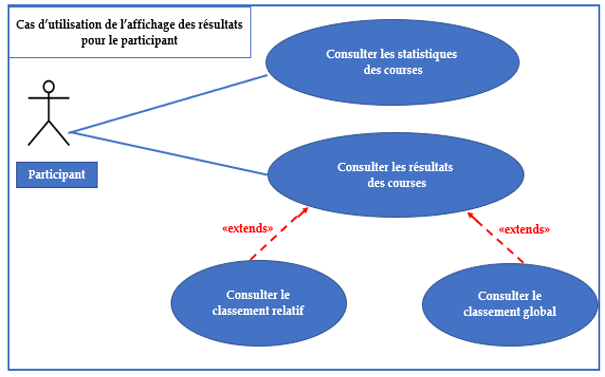
\includegraphics[scale=0.9]{img/Diagramme_cas_utilisation_consultation_resultats.png}
	   \caption {Diagramme de cas d’utilisation de l’affichage des résultats pour les participants}
\end{figure}
\subsection {Diagramme des classes}
\subsubsection{Définition}
Le diagramme de classes est un schéma utilisé en génie logiciel pour présenter les classes et les interfaces des systèmes ainsi que les différentes relations entre celles-ci. Ce diagramme fait partie de la partie statique d'UML car il fait abstraction des aspects temporels et dynamiques.

\subsubsection{Les classes}
Le diagramme des classes du projet est illustré par la figure présente page suivante.

\begin{sidewaysfigure}
	   \center
	   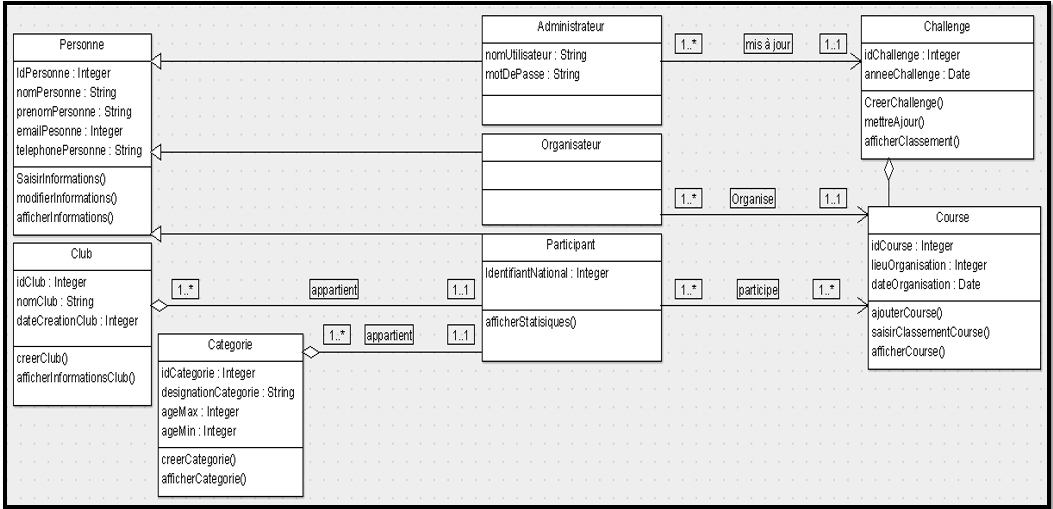
\includegraphics[scale=0.8]{img/Diagramme_classes.png}
	   \caption {Diagramme des classes du projet}
\end{sidewaysfigure}

Le diagramme des classes du projet, figurant dans la capture d’écran précédente est composé de huit classes répertoriées comme suit :
\begin{itemize} 
 	\item La classe Personne qui est une classe abstraite dont héritent les classes Participant, Organisateur et Administrateur. Cette classe possède les attributs suivants : identifiant de la personne, son nom, son prénom, son email et son numéro de téléphone.
 	\item La classe Participant qui est une classe fille de la classe Personne qui possède, en plus des attributs hérités de la classe Personne, un attribut identifiant national qui va permettre de pallier au problème des homonymes dans l’avenir si une migration des données vers une base de données nationale est projetée.
 	\item La classe Administrateur qui est une classe fille de la classe Personne ayant, en plus des attributs hérités de la classe Personne, des attributs d’authentification (nom utilisateur et mot de passe) permettant à l’administrateur de s’authentifier. 
 	\item La classe Organisateur qui hérite ses attributs et ses méthodes de la classe Personne.
 	\item La classe Club : elle représente le club auquel appartient le participant, avec les attributs suivants : nom et la date de création du club.
 	\item La classe Challenge : est une classe qui symbolise les challenges, elle est caractérisée par les attributs : nom, et l’année de création du challenge.
 	\item La classe Course : contient les informations relatives aux courses organisées (la date de l’organisation de la course, le nombre de participants, le lieu d’organisation).
 	\item La classe Catégorie : Comme les participants dans les courses appartiennent à des catégories différentes, il est nécessaire d’implémenter une classe qui stocke les informations inhérentes à chaque catégorie. 
\end{itemize}
\subsubsection{Les relations entres les classes}
Les différentes classes du diagramme peuvent être liées par des types de relations variées selon le type de relation entre elles et également selon le nombre d’instances générées de chacune d’entre elles lors de l’exécution. Ainsi cet axe est dédié pour détailler ces relations.
\begin{itemize} 
 	\item Les classes Participant, Organisateur et Administrateur sont des classes filles de la classe Personne, c’est-à-dire qu’elles héritent des méthodes et des attributs de celle-ci. Il reste à préciser que les méthodes seront surchargées ou redéfinies selon chaque classe.
 	\item La classe Club et la Classe Participant sont liées par une relation d’agrégation c’est-à-dire que plusieurs participants appartiennent à un club et une personne adhère à un seul Club.
 	\item La classe Participante est liée à la classe Course par une relation d’association, en effet un participant peut participer à plusieurs courses et une course est ouverte à plusieurs personnes.
 	\item Une Course doit être insérer dans un seul challenge, vu que la classe Course et Challenge sont liées par une relation d’association avec les cardinalités 1..1 du coté de la course.
 	\item Un participant appartient à une et une seule catégorie, alors qu’une catégorie peut contenir plusieurs participants. 
	\item Une course est organisée par un seul Organisateur et un organisateur peut organiser plusieurs courses.
 	\item Un administrateur peur mettre à jour plusieurs Challenge, et un Challenge est obligatoirement par un seul administrateur.
 	\item Les résultats d’une course figurent dans un seul fichier Challenge et un challenge peut contenir plusieurs courses. 
\end{itemize} 


\subsection {Le diagramme d’activités}
\subsubsection{Définition}
Les diagrammes d'activités permettent de mettre l'accent sur les traitements. Ils sont donc particulièrement adaptés à la modélisation du cheminement et de contrôle des flots de données. 
\subsubsection{Le diagramme d'activité du projet}
\begin{sidewaysfigure}
	   \center
	   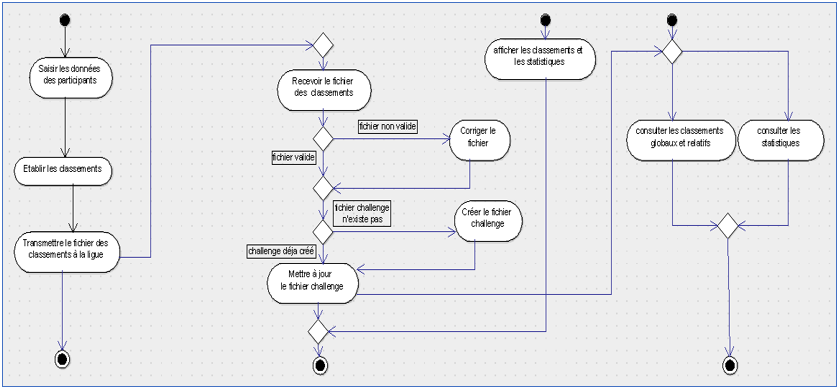
\includegraphics[scale=0.9]{img/Diagramme_activites.png}
	   \caption {Le diagramme d’activités du projet}
\end{sidewaysfigure}

Le diagramme illustré dans la figure ci-dessous montre le diagramme d’activités du projet. En effet, il représente les événements déclencheurs des différents processus. Également, il illustre les différentes tâches exécutées d’une manière séquentielle. 